\documentclass[12pt,a4paper]{article}
\usepackage[utf8]{inputenc}
\usepackage[german]{babel}
\usepackage[T1]{fontenc}
\usepackage{times}
\usepackage{graphicx}
\usepackage{url}
\usepackage[dvipsnames]{xcolor}
\usepackage{setspace}
\usepackage{enumerate}
\usepackage{pbox}
\usepackage{amsmath}
\usepackage{amsfonts}
\usepackage{amssymb}
\usepackage{stmaryrd}
\newcommand{\red}[1]{\textcolor{red} {#1}}
\newcommand{\blue}[1]{\textcolor{blue} {#1}}
\newcommand{\green}[1]{\textcolor{ForestGreen} {#1}}
\newcommand{\yellow}[1]{\textcolor{yellow} {#1}}
\newcommand{\nl}{\\[0.1cm]}
\newcommand{\ra}{$\rightarrow$ }
\newcommand{\ont}{\mathcal{O}}
\newcommand{\ip}{^\mathcal{I}}
\newcommand{\sse}{\sqsubseteq}
\newcommand{\sand}{\sqcap}
\newcommand{\sor}{\sqcup}
\title{Logic-based Ontology Engineering}
\author{Henrik Tscherny}
\begin{document}
\maketitle
\tableofcontents

\section{Description Logic\\Attribute Language with Concepts (ALC)}
Description logics (DLs) are a \textit{decidable} subset of first-order logic. They are restricted to \textit{unary and binary predicates} .\\
\subsection{Vocabulary}
\begin{itemize}
\item C: Concepts/Classes/Categories \ra Person(x) is the set of all elements which are a person
\begin{itemize}
\item Concepts can be defined inductively, if C and D are concepts then:
\item \begin{tabular}{c c c c c c}
\textit{Name:} & top & bottom & conjunction & disjunction & negation\\
\textit{Syntax:} & $\top$ & $\bot$ & $C\sqcap D$ & $C\sqcup D$ & $\neg C$\\
\textit{Semantics:} & $\Delta^\mathcal{I}$ & $\emptyset$ & $C^\mathcal{I} \cap D^\mathcal{I}$ & $ C^\mathcal{I} \cup D^\mathcal{I}$ & $\Delta^\mathcal{I} \setminus C^\mathcal{I}$
\end{tabular}
\item Example: Plant $\sqcap$ Tree \ra set of objects being a plant and a tree
\item if C is a concepts and r is a role the following are also concepts (describes \textit{outgoing role connections}):
\item \begin{tabular}{c c c}
\textit{Name:} & existential restriction & value restriction\\
\textit{Syntax:} & $\exists r.C$ & $\forall r.C$\\
\textit{Semantics:} & $\{d\,|\, \exists e.(d,w) \in  r^\mathcal{I} \land e \in C^\mathcal{I}\}$ & $\{d\,|\, \forall e.(d,e) \in r^\mathcal{I} \rightarrow e \in C^\mathcal{I} \}$
\end{tabular}
\item Example: $\exists \,isSpicy.Food \;=\; \exists y.(isSpicy(x,y) \land Food(y))$\\\ra spicy food exists
\item Example 2: $\forall \,isPlant.Tree \;=\; \forall y.(isPlant(x,y) \rightarrow Tree(y))$\\\ra all trees are plants
\item \textit{size} of a concept:
\begin{itemize}
\item size($A$) = size($\top$) = size($\bot$) = \blue{1}
\item size($C\sqcap D$) = size($C\sqcup D$) = \blue{1 + size(C) + size(D)}
\item size($\neg C$) = size($\exists r.C$) = size($\forall r.C$) = \blue{1 + size(C)}\\\ra \textbf{the number of $\exists,\,\forall,\,\neg,\,\sqcap,\,\sqcup,\,\top,\,\bot$ + 'basic' concepts}
\item Example: size($\exists r.(\exists s.A\sqcap \exists r.\exists s.\top)$) = 7
\end{itemize}
\item \textit{role depth} of a concept:

\begin{itemize}
\item rd($A$) = rd($\top$) = rd($\bot$) = \blue{0}
\item rd($\neg C$) = \blue{rd(C)}
\item rd($C\sqcap D$) = rd($C\sqcup D$) = $\blue{max\{rd(C),rd(D)\}}$
\item rd($\exists r.C$) = rd($\forall r.C$) = $\blue{1+rd(C)}$\\\ra \textbf{maximal nesting depth of role restrictions in the concept}
\item Example: rd($\exists r. (\exists s.A\sqcap \exists r.\exists s.\top)$) = 3
\end{itemize}
\item if $C \sse_\ont D$ then C is \blue{more specific} than D, D is \blue{more general} than C

\end{itemize}
\item R: Roles/Relations/Properties/Attributes \ra likes(x,y) is the set of all pairs, where x likes y
\begin{itemize}
\item only unary and binary relations \ra n-ary relations can be transformed into unary and binary relations with \blue{reification}
\end{itemize}
\item I: Objects/Individuals \ra represents a constant in first-order logic, like a TOM, a specific person
\end{itemize}
\flushleft
\subsection{Interpretations}
A DL \textit{interpretation} is a tuple $\mathcal{I} = (\Delta^\mathcal{I}, \cdot^\mathcal{I})$, where:
\begin{itemize}
\item $\Delta^\mathcal{I}$ is the \textbf{domain} of $\mathcal{I}$ ($\Delta^\mathcal{I} \neq \emptyset)$
\item $\cdot^\mathcal{I}$ is the \textbf{interpretation function}
\begin{itemize}
\item each $A\in C$ is interpreted as a set $A^\mathbb{I} \subseteq \Delta^\mathcal{I}$
\item each $r\in R$ is interpreted as a binary relation $r^\mathcal{I} \subseteq \Delta^\mathcal{I} \times \Delta^\mathcal{I}$
\item each $a\in I$ is interpreted a an element $a^\mathcal{I} \in \Delta^\mathcal{I}$
\end{itemize}
\item Interpretations can be represented as labeled graphs like:\\
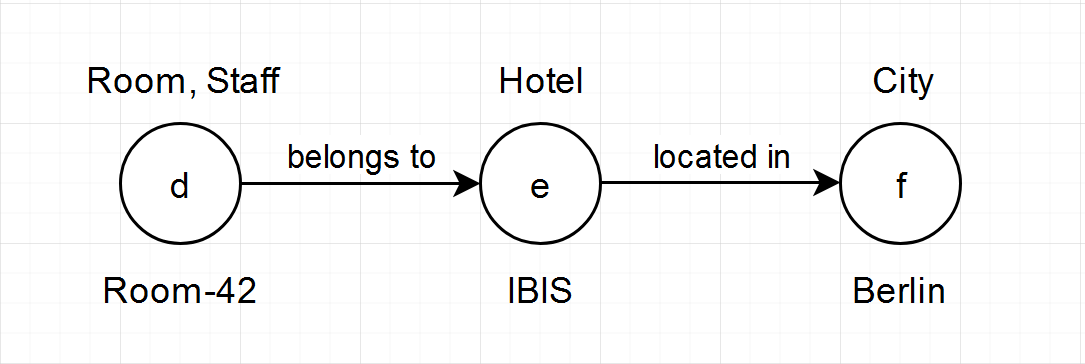
\includegraphics[scale=0.35]{./resources/alc_graph1.png}
\item axioms can be used to restrict the set of interpretations
\item every interpretation is a model of $\emptyset$
\end{itemize}
\flushleft
\subsection{Axioms}
\begin{itemize}
\item \textit{general concept inclusion (CGI)}
\begin{itemize}
\item Syntax: $C\sse D$
\item Semantics: $\mathcal{I} \models C \sse D \Leftrightarrow C\ip \subseteq D\ip$
\item Lecture $\sse$ Course
\end{itemize}
\item \textit{equivalence axiom}
\begin{itemize}
\item $C\equiv D \Leftrightarrow C \sse D \sand D \sse C$
\end{itemize}
\item \textit{concept definitions}
\begin{itemize}
\item $A \equiv D$, where A is a concept name
\item Example: Tutor $\equiv$ Person
\end{itemize}
\item \textit{Assertions/Facts}
\begin{itemize}
\item \begin{tabular}{c c c}
\textit{Name:} & concept assertion & role assertion\\
\textit{Syntax:} & $a:C$ & $(a,b):r$\\
\textit{Semantics:} & $a\ip \in C\ip$ & $(a\ip,b\ip)\in r\ip$
\end{tabular}
\item Example concept assertion: Room-42:Room
\item Example role assertion: (Room-42, IBIS):belongsTo
\end{itemize}
\item \textit{closure axiom}\begin{itemize}
\item define the range/scope of a relation
\item setting the scope of a description under the open world assumption
\item Example: Cow $\sse\forall$ eats.(Grass $\sor$ Grain)
\end{itemize}
\item \textit{covering axiom}
\begin{itemize}
\item (partial) definition with a disjunction on the right
\item can be used to cover not explicitly stated informations
\item Example: Person $\equiv$ Man $\sor$ Woman $\sor$ Diverse
\end{itemize}
\item \textit{disjointness axiom}
\begin{itemize}
\item can be used to separate to concepts from each other
\item Example: Animal $\sse\neg$ Plant
\end{itemize}
\end{itemize}

\subsection{Ontologies}
An ontology is a set $\mathcal{O = A\cup T}$, where:
\begin{itemize}
\item \blue{ABox} $\mathcal{A}$, finite set of assertion/facs (ABox hold the 'data')
\item \blue{TBox} $\mathcal{T}$, finite set of general concept inclusions (TBox hold the 'knowledge')
\item Example:\begin{itemize}
\item $\mathcal{O=A\cup T}$
\item $\mathcal{A} = \{$Room-42$:$Room$,($Room-42$,$IBIS$):$belongsTo$,$\\$($IBIS$, $Berlin$):$locatedIn$\}$
\item $\mathcal{T} = \{$Room$ \sse \neg $City$, $Hotel$ \sse \neg $Room$\}$
\item $C(\mathcal{O}) = \{$Room$, $Hotel$, $City$\}$\\$R(\mathcal{O}) = \{$belongsTo$, $locatedIn$\}$\\$I(\mathcal{O}) = \{$Room-42$, $IBIS$, $Berlin$\}$
\end{itemize}
\item an ontology is \textbf{inconsistent} iff $\mathcal{O} \models \top \sse \bot$
\item if a ontology is consistent the \blue{ABox} is irrelevant for checking satisfiability and subsumption
\item a \blue{TBox $\mathcal{T}$} is called \green{acyclic} if:
\begin{itemize}
\item each concept name A has at most one definition $A \equiv C_A \in\mathcal{T}$
\item the \textit{depends on} relation is acyclic \ra A \textit{depends on} B if B occurs in the definition $C_A$ of A in $\mathcal{T}$
\end{itemize}
\item the \blue{expansion} of C wrt. to an acyclic TBox $\mathcal{T}$ is to exhaustively replace all defined concept names in C by their definitions
\end{itemize}

\subsection{Reasoning}
Reasoning allows to entail information from an ontology
\begin{itemize}
\item reasoning for acyclic ALC TBoxes is in \green{PSpace}, general ALC reasoning is in \green{ExpTime}
\item $\mathcal{O} \text{ \blue{entails} an axiom } \alpha(\blue{\mathcal{O \models \alpha}}) \text{ if every model of } \mathcal{O} \text{ is also a model of }\alpha$
\begin{itemize}
\item \begin{tabular}{c c c}
C is \green{subsumed} by D & $\mathcal{O} \models C \sse D$ & $C\sse_\mathcal{O}D$\\
C is \green{equivalent} to D & $\mathcal{O} \models C \equiv D$ & $C\equiv_\mathcal{O}D$\\
C is \green{strictly subsumed} by D & $C \sse_\mathcal{O} \land C \not\equiv_\mathcal{O} D$ & $C\sqsubset_\mathcal{O}D$\\
C and D are \green{disjoint} & $\mathcal{O} \models C \sand D \sse \bot$ & $-$
\end{tabular}\\
\centering
(everything wrt. to $\mathcal{O}$)
\end{itemize}
\item $\mathcal{O} \models a:C$, a is an \blue{instance} of C
\item $\ont \not\models C \sse \bot$, C is \blue{satisfiable}
\item If all concept names in $\ont$ are satisfiable, then $\ont$ in \blue{coherent}
\item \blue{classification} is the task of computing all entailments of the form $\ont \models A \sse B,\; A,B\in C$
\item \blue{materialization} is the task of computing all entailments of the form $\ont \models a:A$ and $\ont \models (a,b):r$, with $(a,b)\in I, A\in C, r\in R$
\item A \blue{tautology} is an axiom that is satisfied by \textit{all} interpretations
\begin{itemize}
\item if $\alpha$ is a tautology, then $\alpha$ is entailed by the empty ontology $\emptyset$ and also entailed by all $\mathcal{ALC}$ ontologies
\item the following are tautologies\\
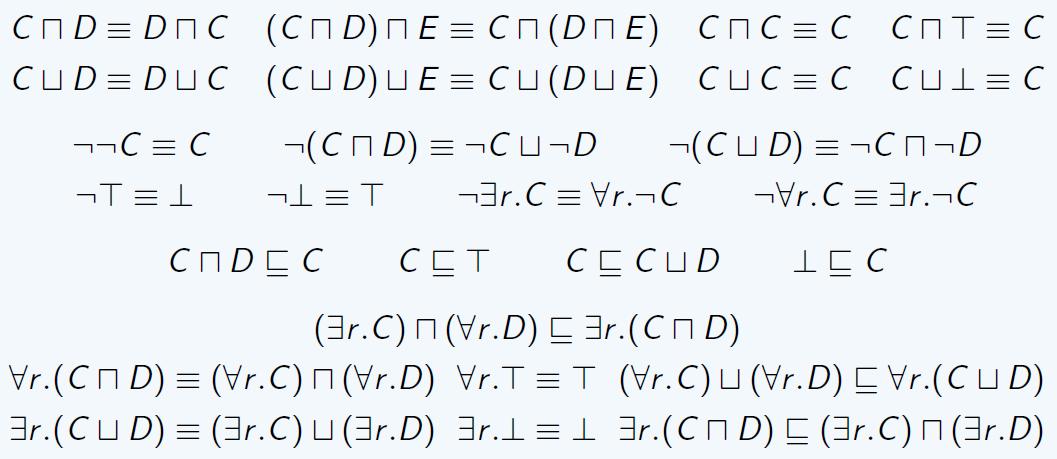
\includegraphics[scale=0.5]{./resources/tautologies.png}
\end{itemize}
\item in \blue{negation normal form (NNF)} negation ($\neg$) is only directory in front of concept names
\item every concept can be expressed in NNF
\item \textit{entailment rules}:
\begin{itemize}
\item $C \sse_\ont D \land D \sse_\ont E \rightarrow C \sse_\ont E$ (\blue{transitivity})
\item $C \sse_\ont D \rightarrow \exists r.C \sse_\ont \exists r.D, \forall r.D, C \sand E \sse_\ont D \sand E \land C \lor R \sse_\ont D \sor E$ (\blue{substitution})
\item $C \sse_\ont D \sand E \leftrightarrow C \sse_\ont D \land C \sse_\ont E$
\item $C \sor D \sse_\ont E \leftrightarrow C \sse_\ont E \land D \sse_\ont E$
\item $C \sand D \sse_\ont E \leftrightarrow C \sse_\ont \neg D \sor E$
\item $C \sse_\ont D \leftrightarrow \neg D \sse_\ont \neg C$ (\blue{contraposition})
\item $C \sand \neg C \sse_\emptyset \bot$ (\blue{contradiction})
\end{itemize}
\item \textit{reasoning with ABoxes}
\begin{itemize}
\item $\ont\models a:C \land C\sse_\ont D \rightarrow \ont \models a:D$
\item $\ont \models a:\top$
\item $\ont\models a:\bot \rightarrow \top \sse_\ont \bot$ ($\ont$ is inconsistent)
\item $\ont \models a:(C\sand D) \leftrightarrow \ont \models a:C \land \ont \models a:D$
\item $\ont\models a:C \lor \ont \models a:D \rightarrow \ont\models a:(C\sor D)$
\item $\ont\models a:C \land \ont \text{ is consistent } \rightarrow \ont \not\models a:\neg C$
\item $\ont \models (a,b):r \land \ont\models b:C \rightarrow \ont \models a:(\exists r.C)$
\item $\ont \models (a,b):r \land \ont \models a:(\forall r.C) \rightarrow \ont\models b:C$\\
\centering
(1-4) hold in both directions
\end{itemize}
\end{itemize}

\subsection{Open World vs. Closed World}
\begin{itemize}
\item in an \red{open-world assumption}, unknown $\neq$ false\\\ra you have to explicitly state that sth. is false
\item in a \red{closed-world assumption}, unknown $=$ false\\\ra you have to explicitly state that sth. is true
\end{itemize}

\section{SROIQ(D)}
More expressive DL then ALC, that is still decidable (reasoning is \green{2-NExpTime-complete})\\
SROIQ(D) stands for:
\begin{itemize}
\item transitive roles (S)
\item complex role axioms (R)
\item nominals (O)
\begin{itemize}
\item \begin{tabular}{c c c}
\textit{Name} & nominal & local reflexivity\\
\textit{Syntax} & $\{a\}$ & $\exists$r.Self\\
\textit{Semantics} & $\{a\ip\}$ & $\{x\,|\, (x,x) \in r\ip\}$\\
\textit{Example} & $\exists$employedBy.$\{$TUDresden$\}$ & $\exists$loves.Self
\end{tabular}
\end{itemize}
\item Inverse roles (I)
\begin{itemize}
\item \begin{tabular}{c c}
\textit{Name} & inverse role\\
\textit{Syntax} & $r^-$\\
\textit{Semantics} & $(r^-)\ip = \{(d,e)\,|\, (e,d)\in r\ip\}$\\
\textit{Example} & belongsTo$^-$
\end{tabular}
\end{itemize}
\item qualified number restrictions (Q)
\begin{itemize}
\item \begin{tabular}{c c c}
\textit{Name} & at-least restriction & at-most restriction\\
\textit{Syntax} & $\geq n r.C$ & $\leq n r.C$\\
\textit{Semantics} & $\{d\,|\, \# \{e\in C\ip \,|\, (d,e)\in r\ip \} \geq n\}$ & $\{d\,|\, \# \{e\in C\ip \,|\, (d,e)\in r\ip \} \leq n\}$\\
\textit{Example} & Student $\sand$ ($\geq$ 2 attends.Lecture) & $\leq$ 1 belongsTo.$\top$
\end{tabular}\\
\centering
(qualifiers e.g. $\leq$ and $\geq$ are optional and only numbers can be used)
\end{itemize}
\item concrete domains (D)
\end{itemize}
\subsection{Structure}
\begin{itemize}
\item In SROIQ(D) an ontology consists of three parts $\ont = \mathcal{A} \cup \mathcal{T} \mathcal{R}$
\item \textit{Assertions}
\begin{itemize}
\item \begin{tabular}{c c c c}
\textit{Name} & equality & inequality & negated role assertion\\
\textit{Syntax} & $a\approx b$ & $a \not\approx b$ & $(a,b):\neg r$\\
\textit{Semantics} & $a\ip$ & $a\ip \neq b\ip$ & $(a\ip,b\ip)\not\in r\ip$\\
\textit{Example} & DD $\approx$ Dresden & $DD\not\approx APB$ & (Ernie, Bert): $\neg$ hasBrother
\end{tabular}
\item all assertions are only syntactic sugar:
\begin{itemize}
\item $a:C \Leftrightarrow \{a\} \sse C$ 
\item $a\approx b \Leftrightarrow \{a\} \sse \{b\}$
\item $a\not\approx b \Leftrightarrow \{a\}\sse \neg \{b\}$
\item $(a,b):r \Leftrightarrow \{a\} \sse \exists r.\{b\}$
\item $(a,b):\neg r \Leftrightarrow \{a\} \sse \forall r.\neg \{b\}$
\end{itemize}
\end{itemize}
\item \textit{Role Axioms} $\rightarrow$ RBox
\item a RBox $\mathcal{R}$ is \blue{regular} if there is a strict partial order $<$ on $R^-(\ont)$ s.d:
\begin{itemize}
\item $r<s \Leftrightarrow r^- < s, \forall r,s \in R^-(\ont)$
\item every role inclusion is of the form:
\begin{itemize}
\item $r\circ r \sse r$
\item $r^- \sse r$
\item $r_1 \circ\cdots\circ r_n \sse r$
\item $\green{r}\circ r_1\circ\cdots\circ r_n \sse r$
\item $r_1\circ\cdots\circ r_n \circ \green{r}\sse r$
\end{itemize}
\end{itemize}
\item role axioms:
\begin{itemize}
\item \begin{tabular}{c c c}
\textit{Name} & \textit{Syntax} & \textit{Meaning}\\
Domain & $Dom(r) \sse C $ & $\exists r.\top \sse C$\\
Range & $Ran(r) \sse C$ & $\exists r^- .\top \sse C, \; \top \sse \forall r.C$\\
Functionality & $Fun(r)$ & $\top \sse \leq 1 r.\top$\\
Reflexivity & $Ref(r)$ & $\top \sse \exists r.Self$\\
\hline
\end{tabular}
\item \begin{tabular}{c c c}
\textit{Name} & role inclusion & complex role inclusion\\
\textit{Syntax} & $r\sse s$ & $s_1 \circ\cdots\circ s_n\sse r$\\
\textit{Semantics} & $s_1\ip\circ\cdots\circ s_n\ip \subseteq r\ip$\\
\hline
\end{tabular}
\item \begin{tabular}{c c c}
\textit{Name} & role disjointness & global reflexivity\\
\textit{Syntax} & $Dis(r,s)$ & $Ref(r)$\\
\textit{Semantics} & $r\ip \cup s\ip = \emptyset$ & $\{(x,x) \,|\, x\in \Delta\ip\}\subseteq r\ip$
\end{tabular}
\item \textit{Additional Axioms}:\\
\begin{tabular}{c c c}
\textit{Name} & \textit{Syntax} &\textit{Defined as}\\
\hline
disjointness & $Dis(C,D)$ & $C\sse \neg D\lor D\sse \neg C \lor C\sand D \sse \bot$\\
role equivalence & $r\equiv s$ & $r\sse s, s\sse r$\\
domain restriction & $Dom(r) \sse C$ & $\top\sse\forall r^- .c \lor \exists r.\top \sse C$\\
range restriction & $Ran(r) \sse C$ & $\top \sse \forall r.C \lor \exists r^-.\top \sse C$\\
role irreflexivity & $Irr(r)$ & $\exists r.Self \sse \bot$\\
role functionality & $Fun(r)$ & $\top \sse \leq 1 r$\\
role symmetry & $Sym(r)$ & $r\sse r^-$\\
role asymmetry & $Asy(r)$ & $Dis(r,r^-)$\\
role transitivity & $Tra(r)$ & $r\circ r\sse r$
\end{tabular}
\end{itemize}
\item \textit{Concrete Domains} $\rightarrow$ $\Delta^D = \mathbb{Z}$, One$^D = 1$, Even$^D = \{...,-2,0,2,...\}$
\item \textit{Attributes}
\begin{itemize}
\item Let $R_C$ be an infinite set of concrete role names (also called \blue{attribute names})
\item extend the definitions of an Interpretation $\mathcal{I}$ to assign each $u\in R_C$ a binary relation $u\ip \subseteq \Delta\ip \times \Delta\ip$
\item Example: (APB/E005, 30):hasSize, Fun(hasSize)
\end{itemize}
\item \textit{Concrete Role Restrictions}
\begin{itemize}
\item \begin{tabular}{c c}
\textit{Name} & (concrete) existential restriction\\
\textit{Syntax} & $\exists u.P$ \\
\textit{Semantics} & $\{d\,|\, \exists v.(d,v)\in u\ip \land v \in P^D\}$\\
\textit{Example} & $\exists$hasSize.Positive,\quad $\exists$hasPrice.$\geq$ 1000 EUR
\end{tabular}
\end{itemize}
\end{itemize}
\section{EL}
Much simpler DL with much lower complexity, EL can be reasoned in \green{PTime}
\begin{itemize}
\item $\mathcal{EL}$ is the sublogic of $\mathcal{ALC}$ that only allows $\top,\sand,\exists r.C$
\item all $\mathcal{EL}$ ontologies are consistent and all concepts within are satisfiable
\item an \blue{Atom} is a concept name or an existential restriction ($At(C) := \{C_1,...,C_n\}$)
\item every concept $C$ is equivalent to a concept of the form $C_1 \sand \cdots \sand C_n$ ($C=\top$ is the empty conjunction with $At(\top) = \emptyset$)
\item in $\mathcal{EL}$ concepts are expressed as \blue{description trees}
\end{itemize}
\subsection{Description Trees}
\begin{itemize}
\item description Tree $T=(V,E,v_0,l)$ with:
\begin{itemize}
\item root node: $v_0$
\item nodes $v\in V$
\item edged $e \in E$
\item labeling function $l(v) \subseteq C$ which assigns each node a finite set of concepts and $l(e) \in R$ assigns each edge role names
\end{itemize}
\item the root node $v_0$ is labeled by $l(v) := At(C) \cap C$
\item for every $\exists r.D \in At(C), \exists (v_0, v_{\exists r.D}) : l(v_0, v_{\exists r.D}) := r$ where $v_{\exists r.D}$ is the root of a \green{copy} of the description tree $T_D$ of D
\item Example: $A \sand \exists r.(A\sand (\exists s.A) \sand B) \sand E s.A$\\
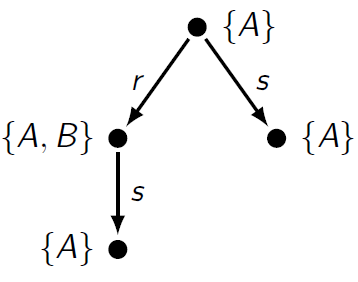
\includegraphics[scale=0.5]{./resources/tree1.png}
\item the tree $T_C$ can be seen as an interpretation whose root satisfies C\\this interpretation is called the \blue{canonical models} of C
\item \textit{Proof} (by induction on the role depth of C):
\begin{itemize}
\item base case ($\red{rd(C) = 0}$):
\begin{itemize}
\item C is a conjunction of concept names and $\top$
\item for every $A\in At(C), A\in l(v_0)$ and thus $v_0 \in A^{\mathcal{I}_C}$
\item consequently, $\displaystyle v_0 \in \bigg(\bigsqcap_{A\in At(C)} A\bigg)^{\mathcal{I}_C} = C^{\mathcal{I}_C}$
\end{itemize}
\item step (\red{rd(C) > 0}:
\begin{itemize}
\item For $D=A \in At(C) \cap C$ the case is as for $rd(C) = 0$
\item Assume $D =\exists r.E\in At(C)$, then $(v_0, v_{\exists r.E}) \in E$, where $l(v_0, v_{\exists r.E}) = r$ and $v_0, v_{\exists r.E}$ is the root in the description three of E
\item $rd(E) < rd(C)$ and by IH, $v_{\exists r.E} \in E^{\mathcal{I}_C}$
\item $(v_0, v_{\exists r.E}) \in r^{\mathcal{I}_C}$, and thus $v_0 \in (\exists r.E)^{\mathcal{I}_C}$
\item We obtain $\displaystyle v_0 \in \bigg( \bigsqcap_{D\in At(C)} D \bigg)^{\mathcal{I}_C} = C^{\mathcal{I}_C}$
\end{itemize}
\end{itemize}
\item homomorphism between description trees $T_1 = (V_1, E_1, v_1, l_1)$, $T_2 = (V_2, E_2, v_2, l_2)$
\begin{itemize}
\item $h: V_1 \rightarrow V_2$
\item $h(v_1) = v_2$
\item $l_1(v) \subseteq l_2(h(v)), \forall v\in V_1$
\item $\forall (v,w) \in E_1\; \exists (h(v), h(w)) \in E_2$ each edge with the same label
\item 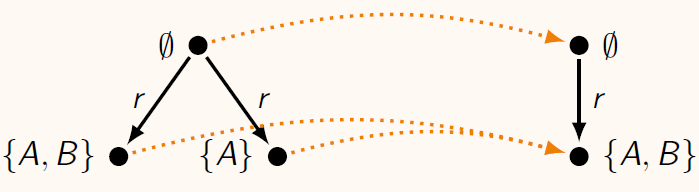
\includegraphics[scale=0.5]{./resources/homomorphism.PNG}
\item for two $\mathcal{EL}$ concepts C, D, the axiom $C\sse D$ is a tautology iff there is a \blue{homomorphism from} $\blue{T_D}$  \blue{to} $\blue{T_C}$
\end{itemize}
\item for two $\mathcal{EL}$ concepts C, D, the axiom $C\sse D$ is a tautology iff $\forall D'\in At(D) \; \exists C'\in At(C): (C',D'\in C \land C'=D') \lor$\\$(C'=\exists r.C'',\,D'=\exists r.D'' \land C''\sse D'') \text{is a tautology}$
\item for two $\mathcal{EL}$ concepts \blue{$C\equiv D \Leftrightarrow T_C \cong T_D$}
\item every $\mathcal{EL}$ concept can be reduced by applying the following rules exhaustively:
\begin{itemize}
\item $C \sand \top \rightarrow C$
\item $C \sand C \rightarrow C$
\item $\exists r.C \sand \exists r.D \rightarrow \exists r.C $ if $ C\sse D$ is a tautology,
\end{itemize}
\end{itemize}
\subsection{Reasoning}
\begin{itemize}
\item \textit{Normal Form of EL TBoxes}
\begin{itemize}
\item A TBox $\mathcal{T}$ is in \blue{normal form} if all CGIs have the form:
\begin{itemize}
\item $A_1 \sand \cdots A_n \sse B$
\item $A \sse \exists r.B$
\item $\exists r.A \sse B$
\end{itemize}
\item if a TBox is not in normal form you may apply those \blue{normalization rules};
\begin{itemize}
\item $C \sse D \sand E \rightarrow C \sse D, \; C\sse E$
\item $C\sse \exists r.\hat{D} \rightarrow C \sse \exists r. A_{\hat{D}},\; A_{\hat{D}} \sse \hat{D}$
\item $\hat{C} \sse \hat{D} \rightarrow \hat{C} \sse A_{\hat{D}}, \; A_{\hat{D}} \sse \hat{D}$
\item $C \sand \hat{D} \sse E \rightarrow \hat{D} \sse A_{\hat{D}}, \; C\sand A_{\hat{D}} \sse E$
\item $\exists r.\hat{C} \sse D \rightarrow \hat{C} \sse A_{\hat{C}} , \; \exists r.A_{\hat{C}} \sse D$
\item $\hat{C}, \hat{D}$ are neither concept names nor $\top$ and $A_{\hat{C}}, A_{\hat{D}}$ is a fresh concept name
\end{itemize}
\end{itemize}
\item with \blue{classification} one can decide several concept subsumptions at once\\(Determine all $A \sse_{\mathcal{T}} B$ where $A,B \in C$)
\begin{itemize}
\item \textit{classification rules}:
\begin{itemize}
\item $\displaystyle\frac{}{A\sse A}$ \blue{(CR1)}
\item $\displaystyle\frac{}{A\sse\top}$ \blue{(CR2)}
\item $\displaystyle\frac{A\sse A_1 \cdots A\sse A_n \quad A_1\sand\cdots\sand A_n \sse B}{A\sse B}$ \blue{(CR3)}
\item $\displaystyle\frac{A\sse \exists r.B \quad B\sse C \quad \exists r.C \sse D}{A\sse D}$ \blue{(CR4)}
\item if the premise is in $\mathcal{T}$ but the conclusion is not, then add the conclusion to $\mathcal{T}$
\end{itemize}
\item every rule adds a new axiom $A \sse B$ $\Rightarrow$ at most \green{quadratic} many inferences
\item the classification terminates in PTime in the size of $\mathcal{T}$
\item classification can also be use to check complex subsumptions $C \sse_{\mathcal{T}} D$, where C, D are not just concept names
\begin{itemize}
\item add the CGIs $A_C \sse C,\; D\sse B_D$ to $\mathcal{T}$, where $A_C, B_D$ are fresh concept names
\item normalize the extended TBox
\item check whether $A_C \sse B_D$ is entailed from it
\end{itemize}
\end{itemize}
\end{itemize}
\section{Ontology Learning}
Extraction knowledge from a source (text, database) and transform it into an ontology
\begin{itemize}
\item \textit{Learning Problem}:
\begin{itemize}
\item $\ont$ a consistent ontology
\item $A\in C$ be the target concept name
\item $E^+ \subseteq I(\ont)$ be a set of positive examples for A
\item $E^- \subseteq I(\ont)$ be a set of negative examples for A
\item \blue{concept learning problem}:
\begin{itemize}
\item $\ont \models a:C_A \forall a\in E^+$
\item $\ont \not\models a:C_A \forall a\in E^-$
\item $\rightarrow$ the ontology models positive but not negative examples
\end{itemize}
\end{itemize}
\item to avoid overfitting we can restrict $C_A$ to be an $\mathcal{ALC}$ concept\\$\rightarrow$a exact solution then may not exist but an approximation does
\item \textit{finding approximate solutions}
\begin{itemize}
\item generate candidates for $C_A$ called \blue{hypotheses}
\item evaluate the hypotheses
\begin{itemize}
\item $fn(C_A) := \# \{a\in E^+ \,|\, \ont \not\models a:C_A\}$ \blue{false negatives}
\item $fp(C_A) := \# \{a\in E^- \,|\, \ont \models a:C_A\}$ \blue{false positives}
\item $\displaystyle acc(C_A) := 1-\frac{fn(C_A)+fp(C_A)}{\#E^+ + \# E^-}$ \blue{accuracy}
\item $\blue{score(C_A)} := acc(C_A) - \beta\cdot size(C_A)$ \quad ($\beta \in [0,1]$ is a parameter)
\item choose the best $C_A$ hypotheses based on score
\item add new concept definition $A\equiv C_A$ to $\ont$
\end{itemize}
\item \textit{how to find a good hypothesis}:
\begin{itemize}
\item Start with $C_A = \top$ which has all positive and negative examples as instances and refine concept iterativly
\item \blue{downward refinement operator $\rho$}
\begin{itemize}
\item $\rho(C) \subseteq \{D\,|\, D \sse_\ont C\}$
\item each $D\in \rho(C)$ is formulated using the signature of $\ont$
\item write $C \rightarrow_\rho D$ if $D\in \rho(C)$
\item $\rightarrow_\rho^*$ is the reflexive transitive closure of $\rightarrow_\rho$
\item D can be reach from C via $\rightarrow_\rho$ if $C\rightarrow_\rho^* D$
\end{itemize}
\item \textit{properties of refinement operator}
\begin{itemize}
\item \textit{(locally) finite}: if $\rho(C)$ is finite for all concepts C
\item \textit{proper}: if $C\rightarrow_\rho D \Rightarrow D \sqsubset_\ont C$
\item \textit{complete}: if $D \sqsubset_\ont \Rightarrow C \rightarrow_\rho^* E$ for some concept $E \equiv_\ont D$
\item \textit{ideal}: if it is finite proper and complete\\
(in each step only finitely many new hypothesis are created which are not equivalent to a previous one and also from which all more specific concepts can be reached from)
\end{itemize}
\item every $\mathcal{ALC}$ ontology has a complete and finite refinement operator but there is no ideal refinement operator
\end{itemize}
\item \textit{refining concepts}
\begin{itemize}
\item define $\downarrow(A)$ as the \blue{lower neighbors} and $\uparrow(A)$ as the \blue{upper neighbors} of A
\item define the \blue{atomic domain} $ADom(r)$ as the unique minimal $A\in C\cup \{\top,\bot\}$ s.d. $\ont \models Dom(r) \sse A$
\item define the \blue{atomic range} $ARan(r)$ similarly
\item instead of $\rho_\top$ (special case of $B=\top$ we define $\rho_B$ relative to a context $B\in C\cup\{\top,\bot\}$
\begin{itemize}
\item $\rho_B(C) := \rho'_B(C) \cup \{\bot,C\sand\top\}$
\item $\rho'_B(\top) := \{C_1 \sor\cdots\sor C_n \,|\, C_1,\cdots,C_n \text{ are of the form (a)-(c)}\}$
\item $\rho'_B(\bot) := \emptyset$
\item $\rho'_B(A) := \{E \,|\, E\in \downarrow (A),\, B\sand E\not\sse_ont \bot\}$
\item $\rho'_B(\neg A) := \{\neg E \,|\, E\in \uparrow (A), \, B\sand \neg E \not\sse_\ont \bot\}$
\item $\rho'_B(\exists r.D) := \{\exists r.E \,|\, E\in \rho_{ARan(r)}(D)\}$
\item $\rho'_B(\forall r.D) := \{\forall r.E \,|\, E\in \rho_{ARan(r)}(D)\}$
\item $\rho'_B(C_1 \sand C_2) := \{C_1\sand E \,|\, E\in \rho_B(C_2)\} \cup \{E\sand C_2 \,|\, E\in \rho_B(C_1)\}$
\item $\rho'_B(C_1 \sor C_2) := \{C_1 \sor E \,|\, E\in \rho_B(C_2)\} \cup \{E\sor C_2 \,|\, E\in \rho_B(C_1\}$
\end{itemize}
\item $\rho_\top$ is \green{complete} for $\mathcal{ALC}$
\item $\rho_\top$ is \green{not proper} for $\mathcal{ALC}$\\($\rho_\top(\exists r.D)$ contains $\exists r.D \sand \top$ which is equivalent to $\exists r.D$)
\end{itemize}
\item $\rho_\top^\sqsubset$ is \green{complete and proper} but not \green{finite}
\end{itemize}
\item \textit{Algorithm}
\begin{itemize}
\item \textbf{Input}: Ontology $\ont$, concept names $A, E^+, E^- \subseteq I(\ont)$, parameter $\beta$
\item \textbf{Output}: A list of candidates for $C_A$
\end{itemize}
\begin{enumerate}
\item initialize search tree with a singe node labeled by $(\top, 0)$
\item \textbf{while} true \textbf{do}:
\begin{itemize}
\item choose a node labeled by $(C,n)$ with maximal $acc(C)-\beta\cdot n$
\item \textbf{for} all $D\in \rho_\top^\sqsubset(C)$ with $size(D) = n+1$ and $D \not\equiv_\ont \bot$ \textbf{do}:
\begin{itemize}
\item create a child node with label $(D,n)$
\end{itemize}
\item change the label of the current node from $(C,n)$ to $(C, n+1)$
\item stop \green{at any time}
\end{itemize}
\item \textbf{return} all concepts in the search tree (ranked by score)
\end{enumerate}
\item the algorithm can be improved further by the use of a \blue{heuristic}
\end{itemize}
\section{Matching/Aligning Ontologies}
Given two ontologies $\ont_1$ and $\ont_2$, an \blue{alignment} $\mathfrak{A}$ is a third ontology that shares the vocabulary of $\ont_1$ and $\ont_2$. $\mathfrak{A}$ contains \blue{bridge axioms} that relate one ore more entities of the ontologies
\begin{itemize}
\item \textit{correspondence} (between $\ont_1$ and $\ont_2$)
\begin{itemize}
\item $(e_1, r, e_2, c)$
\begin{itemize}
\item $e_1$ is in $\ont_1$ and $e_2$ is in $\ont_2$
\item either $e_1, e_2 \in C,\; e_1,e_2\in R,\; \text{or} \; e_1,e_2 \in I$ 
\item $r\in\{\equiv,\sse,\sqsupseteq, \bot, \between\}$
\item $c\in [0,1]$ is a \blue{confidence value}
\end{itemize}
\item Example: (ont1:Arm,$\equiv$,ont2:Arm,0.95)
\end{itemize}
\item similarity can be measured using a \blue{similarity measure} $\sigma M_1 \times M_2 \rightarrow [0,1]$\\(the closer the value is to 1 to more similar are $m_1$ and $m_2$)
\item concept name similarity can be derived from other similarity measures
\begin{itemize}
\item given $f_1: N_1\rightarrow M_1$ and $f_2: \rightarrow M_2$, the \blue{similarity measure induced by $\sigma, f_1, \text{and } f_2$} is $\sigma': N_1 \times N_2 \rightarrow [0,1], \text{where } \sigma'(n_1, n_2) := \sigma(f_1(n_1),f_2(n_2))$
\item Example: $\sigma'$(C20480, GO\_0009987) := $\sigma$("Cellular Process", "cellular process") = 1
\end{itemize}
\item the \blue{distance measure} $\delta$ induced by $\sigma$ is $\delta: M_1 \times M_2 \rightarrow [0,1]$, defined by $\delta(m_1, m_2) := 1-\sigma(m_1, m_2)$\\(similarity and distance measure contain the same information, its only for convenience)
\item \textit{other distance/similarity measures}:
\begin{itemize}
\item \blue{hamming distance}: $\displaystyle\delta(v,w) := \frac{1}{m}\cdot \vert \{i\in \{1,...,n\}\,|\, v_i \neq w_i\}\vert$
\item \blue{substring similarity}: $\displaystyle\sigma(v,w) := \frac{\vert u \vert}{m}$, where $u$ is the longest common substring of $v$ and $w$
\item \textbf{n-gram similarity}: $\displaystyle\sigma(v,w) := \frac{\vert n-gram(v) \cap n-gram(w)\vert}{m-n+1}$, where $n-gram(v)$ is the set of $n$-letter substrings of $v$
\item \blue{levenshtein (edit) distance}: minimal number of (insert, delete, replace) operations to get from $w$ to $v$ (divided by $m$)
\end{itemize}
\item similarity measures can be combined
\begin{itemize}
\item sequentially:\\
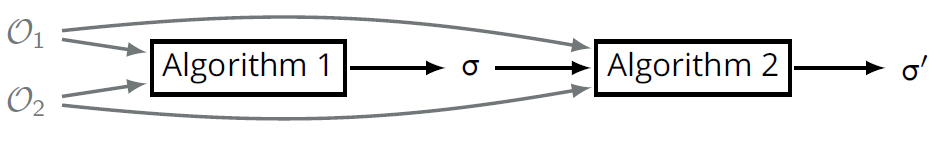
\includegraphics[scale=0.4]{./resources/sequential.png}
\item parallel:\\
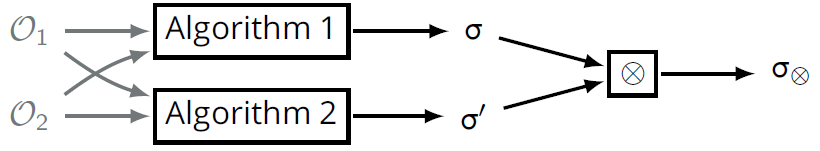
\includegraphics[scale=0.4]{./resources/parallel.png}
\end{itemize}
\item similarity measures can be aggregated (by an \blue{aggregation operator} $\otimes$)
\begin{itemize}
\item weighted sum
\item weighted product
\item \blue{triangular norm} (t-norm) $\otimes: [0,1]\times[0,1]\rightarrow[0,1]$ that is associative, commutative, monotone and has neutral element 1
\item \blue{triangular conorm} (t-conorm) like t-norm but with neutral element 0
\end{itemize}

\item similarity can also be defined for concepts\\
\begin{itemize}
\item \blue{directed similarity} between to Concepts C, D
\begin{itemize}
\item $\displaystyle = \sigma_d(C,D) := \begin{cases} \sigma'(C,D), & C,D \in C\\\sigma'(r,s)\cdot (\beta +(1-\beta\cdot\sigma_d(E,F)), & C=\exists r.E \land D= \exists s.F\\ \displaystyle\min_{D'\in At(D)} \max_{C'\in At(C)} \sigma_d(C',D'),& \vert At(C) \vert > 1 \lor \vert At(D) \vert > 1\\ 1, & At(D)=\emptyset\\ 0, & \text{otherwise}\end{cases}$
\item $\delta_d(C,D)$ measures how C is subsumed by D
\end{itemize}
\item \blue{undirected similarity}
\begin{itemize}
\item $\sigma_u(C,D) := \sigma_d(C,D) \otimes \sigma_d(D,C)$
\item $\otimes$ is a commutative aggregation operator
\end{itemize}
\end{itemize}
\item A similarity should be \blue{equivalence invariant}: $\sigma(\exists r.B, \exists s.D)$ as a function $\sigma'(B,D)$ if $B \equiv_\ont C$, then $\sigma(\exists r.B, \exists s.D)$ should be equal to $\sigma(\exists r.C, \exists s.D)$
\item \textit{from similarity to alignment}
\begin{itemize}
\item given a similarity measure, each concept may be similar to multiple concepts but we only want the best ones
\item \textit{Threshold-based methods} ($\tau \in [0,1]$)
\begin{itemize}
\item \blue{hard threshold}: $\sigma(A,B) \geq \tau$
\item \blue{delta threshold}: $\displaystyle\sigma(A,B) \geq \max_\sigma - \tau$ with $\max_\delta := \max_{A',B'}\{\sigma(A',B')\}$
\item \blue{proportional threshold}: $\sigma(A,B) \geq \tau\cdot\max_\sigma$
\item \blue{percentage threshold}: it is among the $\tau\cdot\vert C(\ont_1)\vert\cdot\vert C(\ont_2)\vert$ correspondences with the highest similarity
\item \blue{normalized threshold}: $\displaystyle \frac{\sigma(A,B)}{\max\{\sigma(A,B')\}} \geq \tau$ and $\displaystyle\frac{\sigma(A,B)}{\max\{\sigma(A',B)\}} \geq \tau$
\end{itemize}
\item sometimes a bijective alignment is needed, where one concept name has exactly one correspondence
\begin{itemize}
\item greedy algorithm
\item maximum weight graph matching
\end{itemize}
\end{itemize}
\end{itemize}

\section{Ontology Maintenance}
\begin{itemize}
\item \textit{Justification}
\begin{itemize}
\item process of finding axioms responsible for erroneous entailment
\item a \blue{justification} $\mathfrak{J}\subseteq \ont$ for an axiom $\alpha$ is:
\begin{itemize}
\item $\mathfrak{J}\models\alpha$
\item $\mathfrak{J}$ is a minimal set with this property $\rightarrow$ $\forall \mathfrak{J}' \subset \mathfrak{J} : \mathfrak{J}'\not\models\alpha$
\end{itemize}
\item a justification provides an explanation for the error $\alpha$
\item computing a single justification is not enough to fix the error because the error may be caused by other clauses for the entailment of $\alpha$
\item \textit{How to compute justifications}
\begin{itemize}
\item \blue{Black-box algorithms}
\begin{itemize}
\item Use reasoner to decide $\ont \models \alpha$ and construct justification as a series of calls to the reasoner
\end{itemize}
\item \blue{Glass-box algorithms}
\begin{itemize}
\item Extend an existing reasoning algorithm for checking $\ont \models\alpha$ to trace the axioms from $\ont$  that are used to derive $\alpha$\\$\rightarrow$ faster but requires more knowledge about the reasoner (harder to implement)
\end{itemize}
\end{itemize}
\item to compute all Justification we need an algorithm to compute a single justification \textit{SingleJustification} (black box algorithm):
\begin{itemize}
\item \textbf{Input}: Ontologies $\ont_f, \ont$, axiom $\alpha$ with $\ont_f \not\models\alpha$ and $\ont_f \cup \ont \models \alpha$
\item \textbf{Output}: A minimal subset $\hat{\ont} \subseteq \ont: \ont_f \cup \hat{\ont}\models\alpha$
\begin{enumerate}
\item \textbf{if} $\vert\ont\vert = 1$ \textbf{then return} $\ont$
\item split $\ont$ int two halves $\ont_1$ and $\ont_2$
\item \textbf{if} $\ont_f \cup \ont_1 \models\alpha$ \textbf{then return} SingleJustification($\ont_f$, $ont_1$, $\alpha$)
\item \textbf{if} $\ont_f \cup \ont_2 \models\alpha$ \textbf{then return} SingleJustification($\ont_f$, $ont_2$, $\alpha$)
\begin{itemize}
\item minimize $\ont_1$ while fixing $\ont_2$, and vice versa
\end{itemize}
\item $\ont'_1$ := \textbf{SingleJustification}($\ont_f\cup\ont_2$,$\ont_1$,$\alpha$)
\item $\ont'_2$ := \textbf{SingleJustification}($\ont_f\cup\ont_1'$,$\ont_2$,$\alpha$)
\item \textbf{return} $\ont'_1 \cup \ont'_2$
\end{enumerate}
\item to compute a single justification for $\alpha$ in $\ont$ we can call \textbf{SingleJustification($\emptyset$, $\ont$, $\alpha$)}
\end{itemize}
\item glass box algorithm (pinpointing)
\begin{itemize}
\item idea: Assign unique labels to axioms in $\ont$, a formula over the labels describes then a subset of $\ont$
\item pinpointing algorithm for $\mathbb{EL}$
\begin{itemize}
\item $\displaystyle \frac{}{(A\sse A)^\text{true}}$ \blue{(CR1)}
\item $\displaystyle \frac{}{(A\sse \top)^\text{true}}$ \blue{(CR2)}
\item $\displaystyle \frac{(A\sse A_1)^{\varphi_1} \cdots (A\sse A_n)^{\varphi_n}\quad (A_1\sand\cdots\sand A_n \sse B)^\varphi}{(A\sse B)^{\varphi_1\land\cdots\land\varphi_n\land\varphi}}$ \blue{(CR3)}
\item $\displaystyle \frac{(A\sse \exists r.B)^{\varphi_1} \quad (B\sse C)^{\varphi_2} \quad (\exists r.C \sse D)^{\varphi_3}}{(A\sse D)^{\varphi_1 \land \varphi_2 \land \varphi_3}}$ \blue{(CR4)}
\end{itemize}
\end{itemize}
\end{itemize}
\end{itemize}
\end{document}
